% ============================================================
% Requiere en el preámbulo de tu documento: amsmath, graphicx, booktabs
% Si tu documento no usa babel/polyglossia en español, asegurate de tener:
%   \renewcommand{\tablename}{Tabla}
%   \renewcommand{\figurename}{Figura}
% Las imágenes parteA_fase.png y parteB_simulacion.png deben estar en la
% misma carpeta que el .tex (o ajustá la ruta en \includegraphics).
% ============================================================


% ---------- INSERTAR DESPUÉS DE LA SUBSECCIÓN 1.2, ANTES DE LA SECCIÓN 2 ----------

\subsection{Análisis de Fase y Ancho de Banda Teórico}

Como complemento al análisis de módulo presentado en la sección anterior, se estudió el comportamiento de la fase $\varphi$ entre la tensión y la corriente del circuito RLC serie, dada por:
\begin{equation}
\varphi(f) = \arctan\left(\frac{\omega L - \dfrac{1}{\omega C}}{R}\right)
\label{eq:fase}
\end{equation}

Dado que en la sección 1.2 se obtuvieron dos valores distintos de inductancia ($L_1 = 46{,}96$ mH a partir de $f_0$, y $L_2 = 35{,}45$ mH a partir del factor de mérito $Q$), se evaluó la ecuación \eqref{eq:fase} para ambos casos, en lugar de asumir arbitrariamente uno de los dos.

Asimismo, en lugar de utilizar la aproximación de banda angosta $BW \approx f_0/Q$, se resolvieron analíticamente las frecuencias de corte exactas a partir de la condición $|Z| = R\sqrt{2}$, que conduce a una ecuación cuadrática en $\omega$ cuyas raíces positivas son:
\begin{equation}
\omega_{1,2} = \frac{\mp R + \sqrt{R^2 + 4L/C}}{2L}
\label{eq:cortes}
\end{equation}

A diferencia de la aproximación usual, la ecuación \eqref{eq:cortes} no asume simetría de $f_1$ y $f_2$ alrededor de $f_0$, lo cual resulta relevante dado el bajo factor de mérito obtenido ($Q \approx 0{,}778$). Cabe notar que, aun así, la diferencia $f_2-f_1$ se reduce algebraicamente de forma exacta a $BW = R/(2\pi L)$, por lo que esta fórmula no constituye en sí misma una aproximación. Los resultados se resumen en la Tabla \ref{tab:bw}.

\begin{table}[h]
\centering
\caption{Frecuencias de corte y ancho de banda teóricos, según el valor de $L$ utilizado, comparados con los valores experimentales.}
\label{tab:bw}
\begin{tabular}{lccc}
\toprule
& $f_1$ [kHz] & $f_2$ [kHz] & $BW$ [kHz] \\
\midrule
$L_1 = 46{,}96$ mH (de $f_0$) & 1{,}69 & 4{,}31 & 2{,}62 \\
$L_2 = 35{,}45$ mH (de $Q$) & 1{,}82 & 5{,}29 & 3{,}47 \\
\textbf{Experimental} & \textbf{1{,}53} & \textbf{5{,}00} & \textbf{3{,}47} \\
\bottomrule
\end{tabular}
\end{table}

La Figura \ref{fig:fase} muestra las curvas de fase teóricas para ambos valores de $L$, junto con las referencias de $f_0$, $f_1$ y $f_2$ experimentales y las asíntotas de $\pm 45^\circ$ correspondientes a las frecuencias de corte ideales.

\begin{figure}[h]
\centering
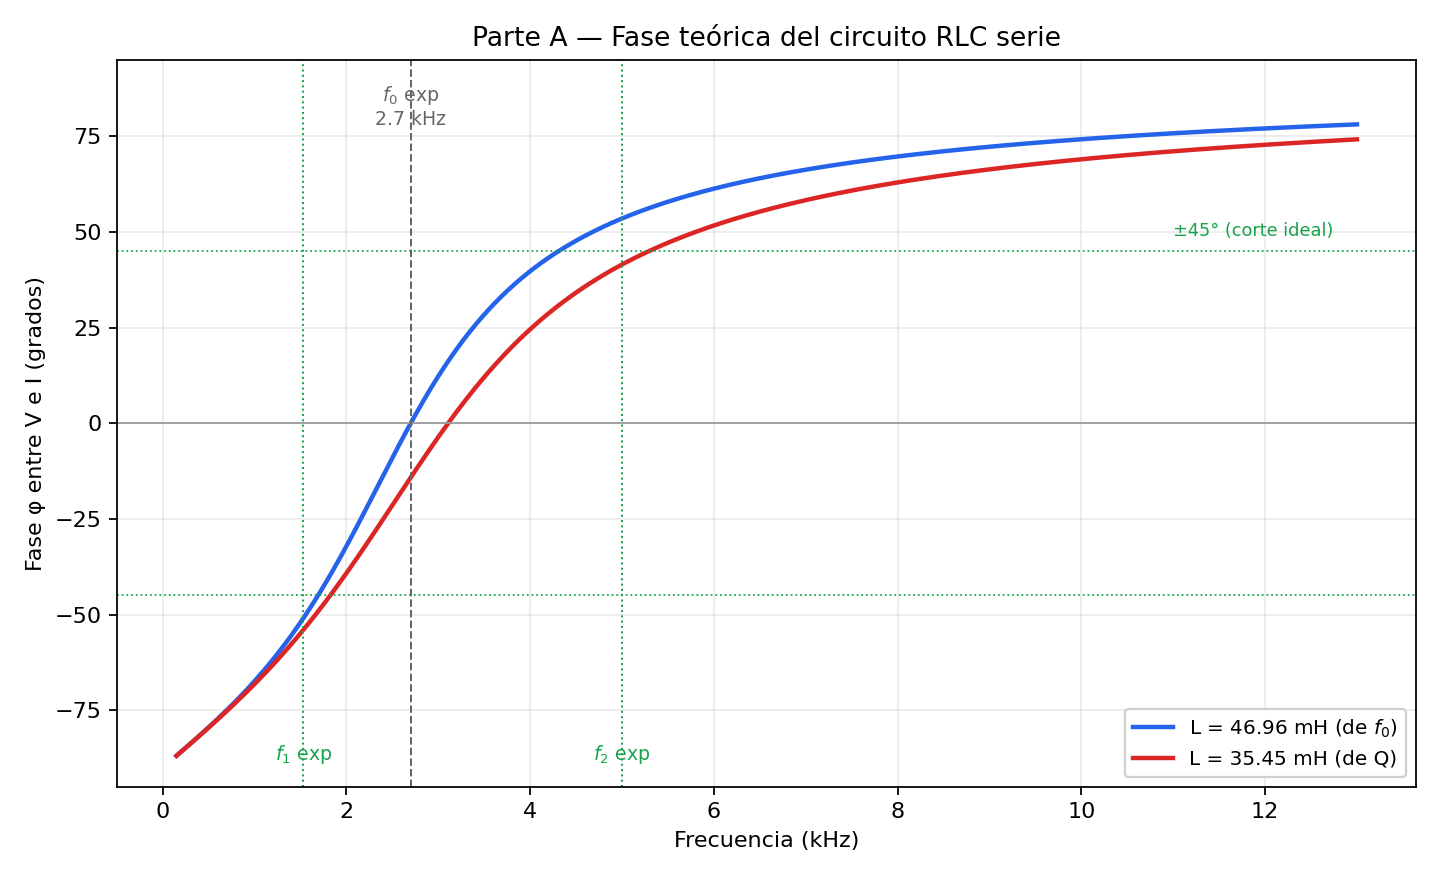
\includegraphics[width=0.85\textwidth]{parteA_fase.png}
\caption{Fase teórica del circuito RLC serie en función de la frecuencia, para los dos valores de $L$ calculados.}
\label{fig:fase}
\end{figure}

Se observa que $L_2$ reproduce casi exactamente el ancho de banda experimental, lo cual es consistente por construcción, ya que dicho valor fue obtenido precisamente a partir de las frecuencias de corte medidas ($f_1$ y $f_2$). El resultado más informativo surge al comparar con $L_1$: al ser calculado de forma independiente, únicamente a partir de la frecuencia de resonancia, predice un ancho de banda teórico un $24\,\%$ más angosto que el medido experimentalmente. Esto indica que la discrepancia entre ambos valores de inductancia, ya señalada en la sección 1.2, no es meramente numérica sino que tiene una consecuencia física directa sobre la selectividad predicha del circuito.

Adicionalmente, se verificó que la relación $f_0^2 = f_1 \cdot f_2$, válida bajo la aproximación de alto $Q$, no se cumple de forma exacta con los datos experimentales ($f_0^2 = 7{,}29 \times 10^6\text{ Hz}^2$ frente a $f_1 f_2 = 7{,}65\times10^6\text{ Hz}^2$, una diferencia del $4{,}9\,\%$), lo cual es coherente con el bajo factor de mérito obtenido y confirma que el circuito se aleja del comportamiento de banda angosta idealizado.


% ---------- INSERTAR DESPUÉS DE LA SUBSECCIÓN 2.2, ANTES DE LA SECCIÓN 3 (CONCLUSIONES) ----------

\subsection{Verificación Mediante Simulación de Circuito}

Con el fin de validar los valores de $r$ y $L$ obtenidos mediante el método geométrico mediante una vía de cálculo independiente, se modeló numéricamente\footnote{Implementado mediante un script en Python, utilizando como entrada los valores de $R$, $r$ y $L$ ya obtenidos.} el circuito como una impedancia serie pura, sin recurrir al Teorema del Coseno utilizado en la sección 2.1:
\begin{equation}
|Z_{total}| = \sqrt{(R+r)^2 + (\omega L)^2}, \qquad |Z_{bobina}| = \sqrt{r^2 + (\omega L)^2}
\label{eq:zsim}
\end{equation}

Utilizando $R = 50\ \Omega$, junto con los valores previamente calculados $r = 49{,}93\ \Omega$ y $L = 222{,}817$ mH, se obtuvo $\omega L \approx 70{,}00\ \Omega$, $|Z_{total}| \approx 122{,}01\ \Omega$ y $|Z_{bobina}| \approx 85{,}98\ \Omega$. A partir de estos módulos de impedancia y de la corriente eficaz medida $I = 105{,}6$ mA, se predijeron las restantes tensiones del circuito mediante la ley de Ohm fasorial, y se contrastaron con los valores leídos directamente en el laboratorio (Tabla \ref{tab:sim}).

\begin{table}[h]
\centering
\caption{Comparación entre los valores medidos en el laboratorio (Tabla 2) y los predichos a partir de la impedancia simulada.}
\label{tab:sim}
\begin{tabular}{lccc}
\toprule
Magnitud & Medido & Predicho & Diferencia \\
\midrule
$V_{total}$ & 12{,}95 V & 12{,}88 V & 0{,}51\,\% \\
$V_R$ & 5{,}36 V & 5{,}28 V & 1{,}49\,\% \\
$V_{zL}$ & 9{,}08 V & 9{,}08 V & $\sim$0\,\% \\
$I$ & 105{,}60 mA & 106{,}14 mA & 0{,}51\,\% \\
\bottomrule
\end{tabular}
\end{table}

La Figura \ref{fig:onda} muestra las formas de onda temporales simuladas de $V_{total}(t)$, $V_R(t)$ e $I(t)$, construidas a partir de las magnitudes medidas y del ángulo de desfase $\varphi \approx 34{,}8^\circ$ calculado en la sección 2.2. Para esta representación temporal fue necesario asumir que los valores leídos en la Tabla 2 corresponden a magnitudes eficaces (RMS), convención estándar de los instrumentos de medición utilizados; dicha suposición afecta únicamente la escala de amplitud de la figura y no las conclusiones numéricas de la Tabla \ref{tab:sim}, que son independientes de esta convención.

\begin{figure}[h]
\centering
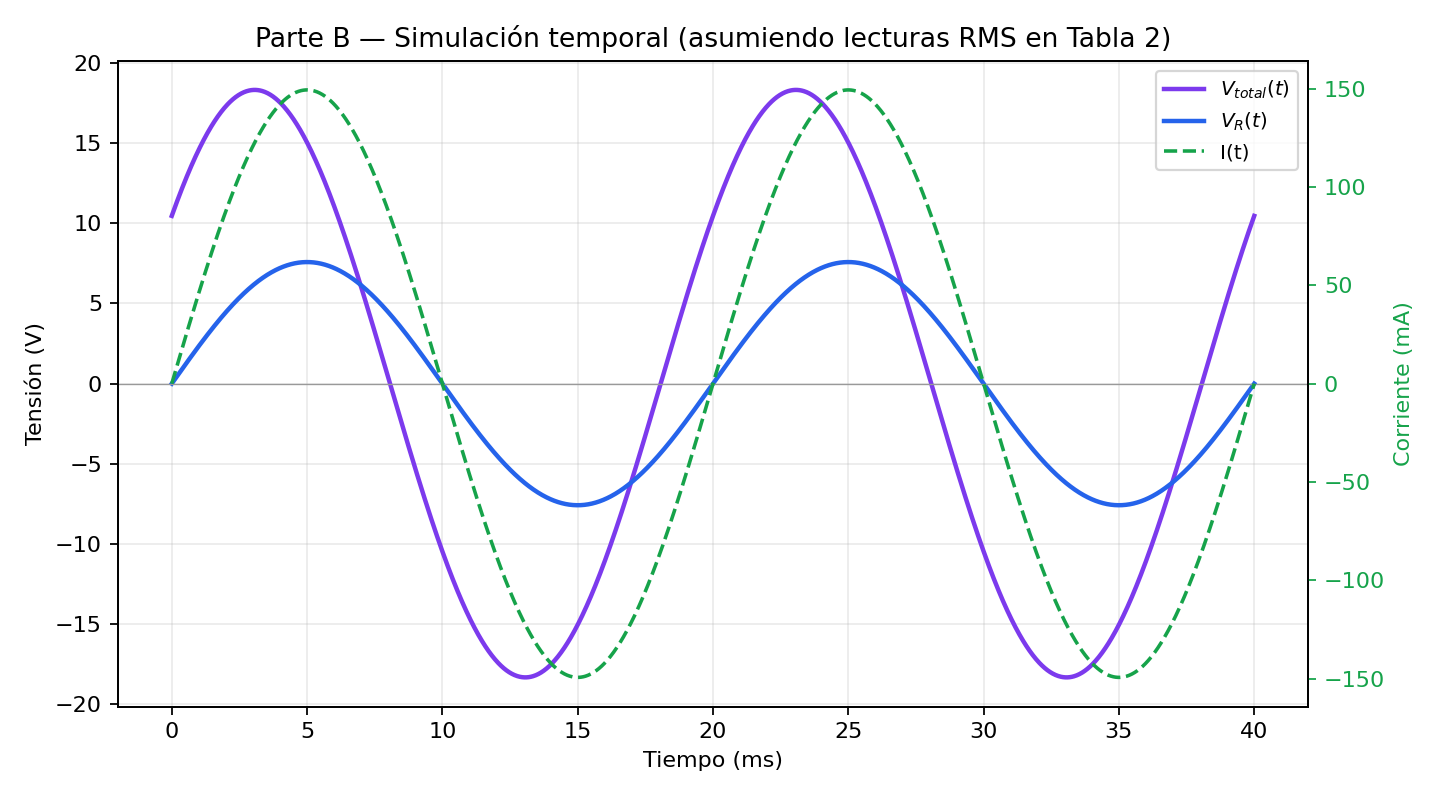
\includegraphics[width=0.85\textwidth]{parteB_simulacion.png}
\caption{Formas de onda simuladas de $V_{total}$, $V_R$ e $I$ para el circuito RL real de la Parte B.}
\label{fig:onda}
\end{figure}

Las diferencias obtenidas, todas inferiores al $1{,}5\,\%$, confirman que los valores de $r$ y $L$ calculados mediante el método fasorial geométrico son consistentes con el cálculo directo de impedancia, lo cual constituye una verificación cruzada independiente del procedimiento utilizado en la sección 2.2. El pequeño residuo remanente es atribuible a la propagación de redondeo a lo largo de la cadena de cálculo ($\cos\varphi \rightarrow V_r, V_L \rightarrow r, L$), y no a un error sistemático del método.
